\chapter{Stacking Methodology}
Initially outlined in \cite{2016MNRAS.457.2391C}, the stacking algorithm involves creating a list of galaxy pairs, which we would expect to see a filament between, and then using those pairs, forming a normalised two-dimensional image, with the galaxies of the pair being placed on two points in the image, and stacking them until the signal to noise is sufficient to be measurable.

The intial problem faced involves generating the galaxy pairs from the Dark Energy Survey redMaGiC Catalogue. The Year 1 Catalogue consists of 0.65 million red-sequence galaxies in the redshift range $0.15 < z < 0.9 $. The algorithm used by the Dark Energy Survey to select these red-sequence galaxies provides redshift estimates of very high quality and very low bias ($\lesssim 0.5$ percent). They also have very low scatter, and a very low rate of catastrophic outliers. The algorithm yields superior photo-z performance than the colour-cut methodology used to definte the Sloan Digital Sky Survey CMASS catalogue \citep{2016MNRAS.461.1431R}. 

Pairs were generated by making use of kD-trees. A generalisation of a binary tree, the kD tree is one where every leaf node is representative of a $k$ dimensional point. Each non-leaf node is one that 'splits' the space into two parts, whereby points to the left of this hyperplane are represented by the left sub-tree, and to the right are represented by the right sub-tree. When we apply this to our galaxy catalogue, we first locate them in 3 dimensional space, by converting their RA, Dec, and redshift into a comoving 3D coordinate. They are then placed in a kD tree, and any pair which has a radial comoving separation of less that $10 h^{-1} $ Mpc, and transverse comoving separation range of $6 - 14 h^{-1} $ Mpc is considered to have a filament \citep{2016MNRAS.457.2391C}.

From this, approximately 340,000 galaxy pairs were constructed with a mean angular separation of $\sim 31.6 $ arcmins, and a mean comoving separation of $11.9 h^{-1}$ Mpc. 
\begin{figure}[h!]
\centering
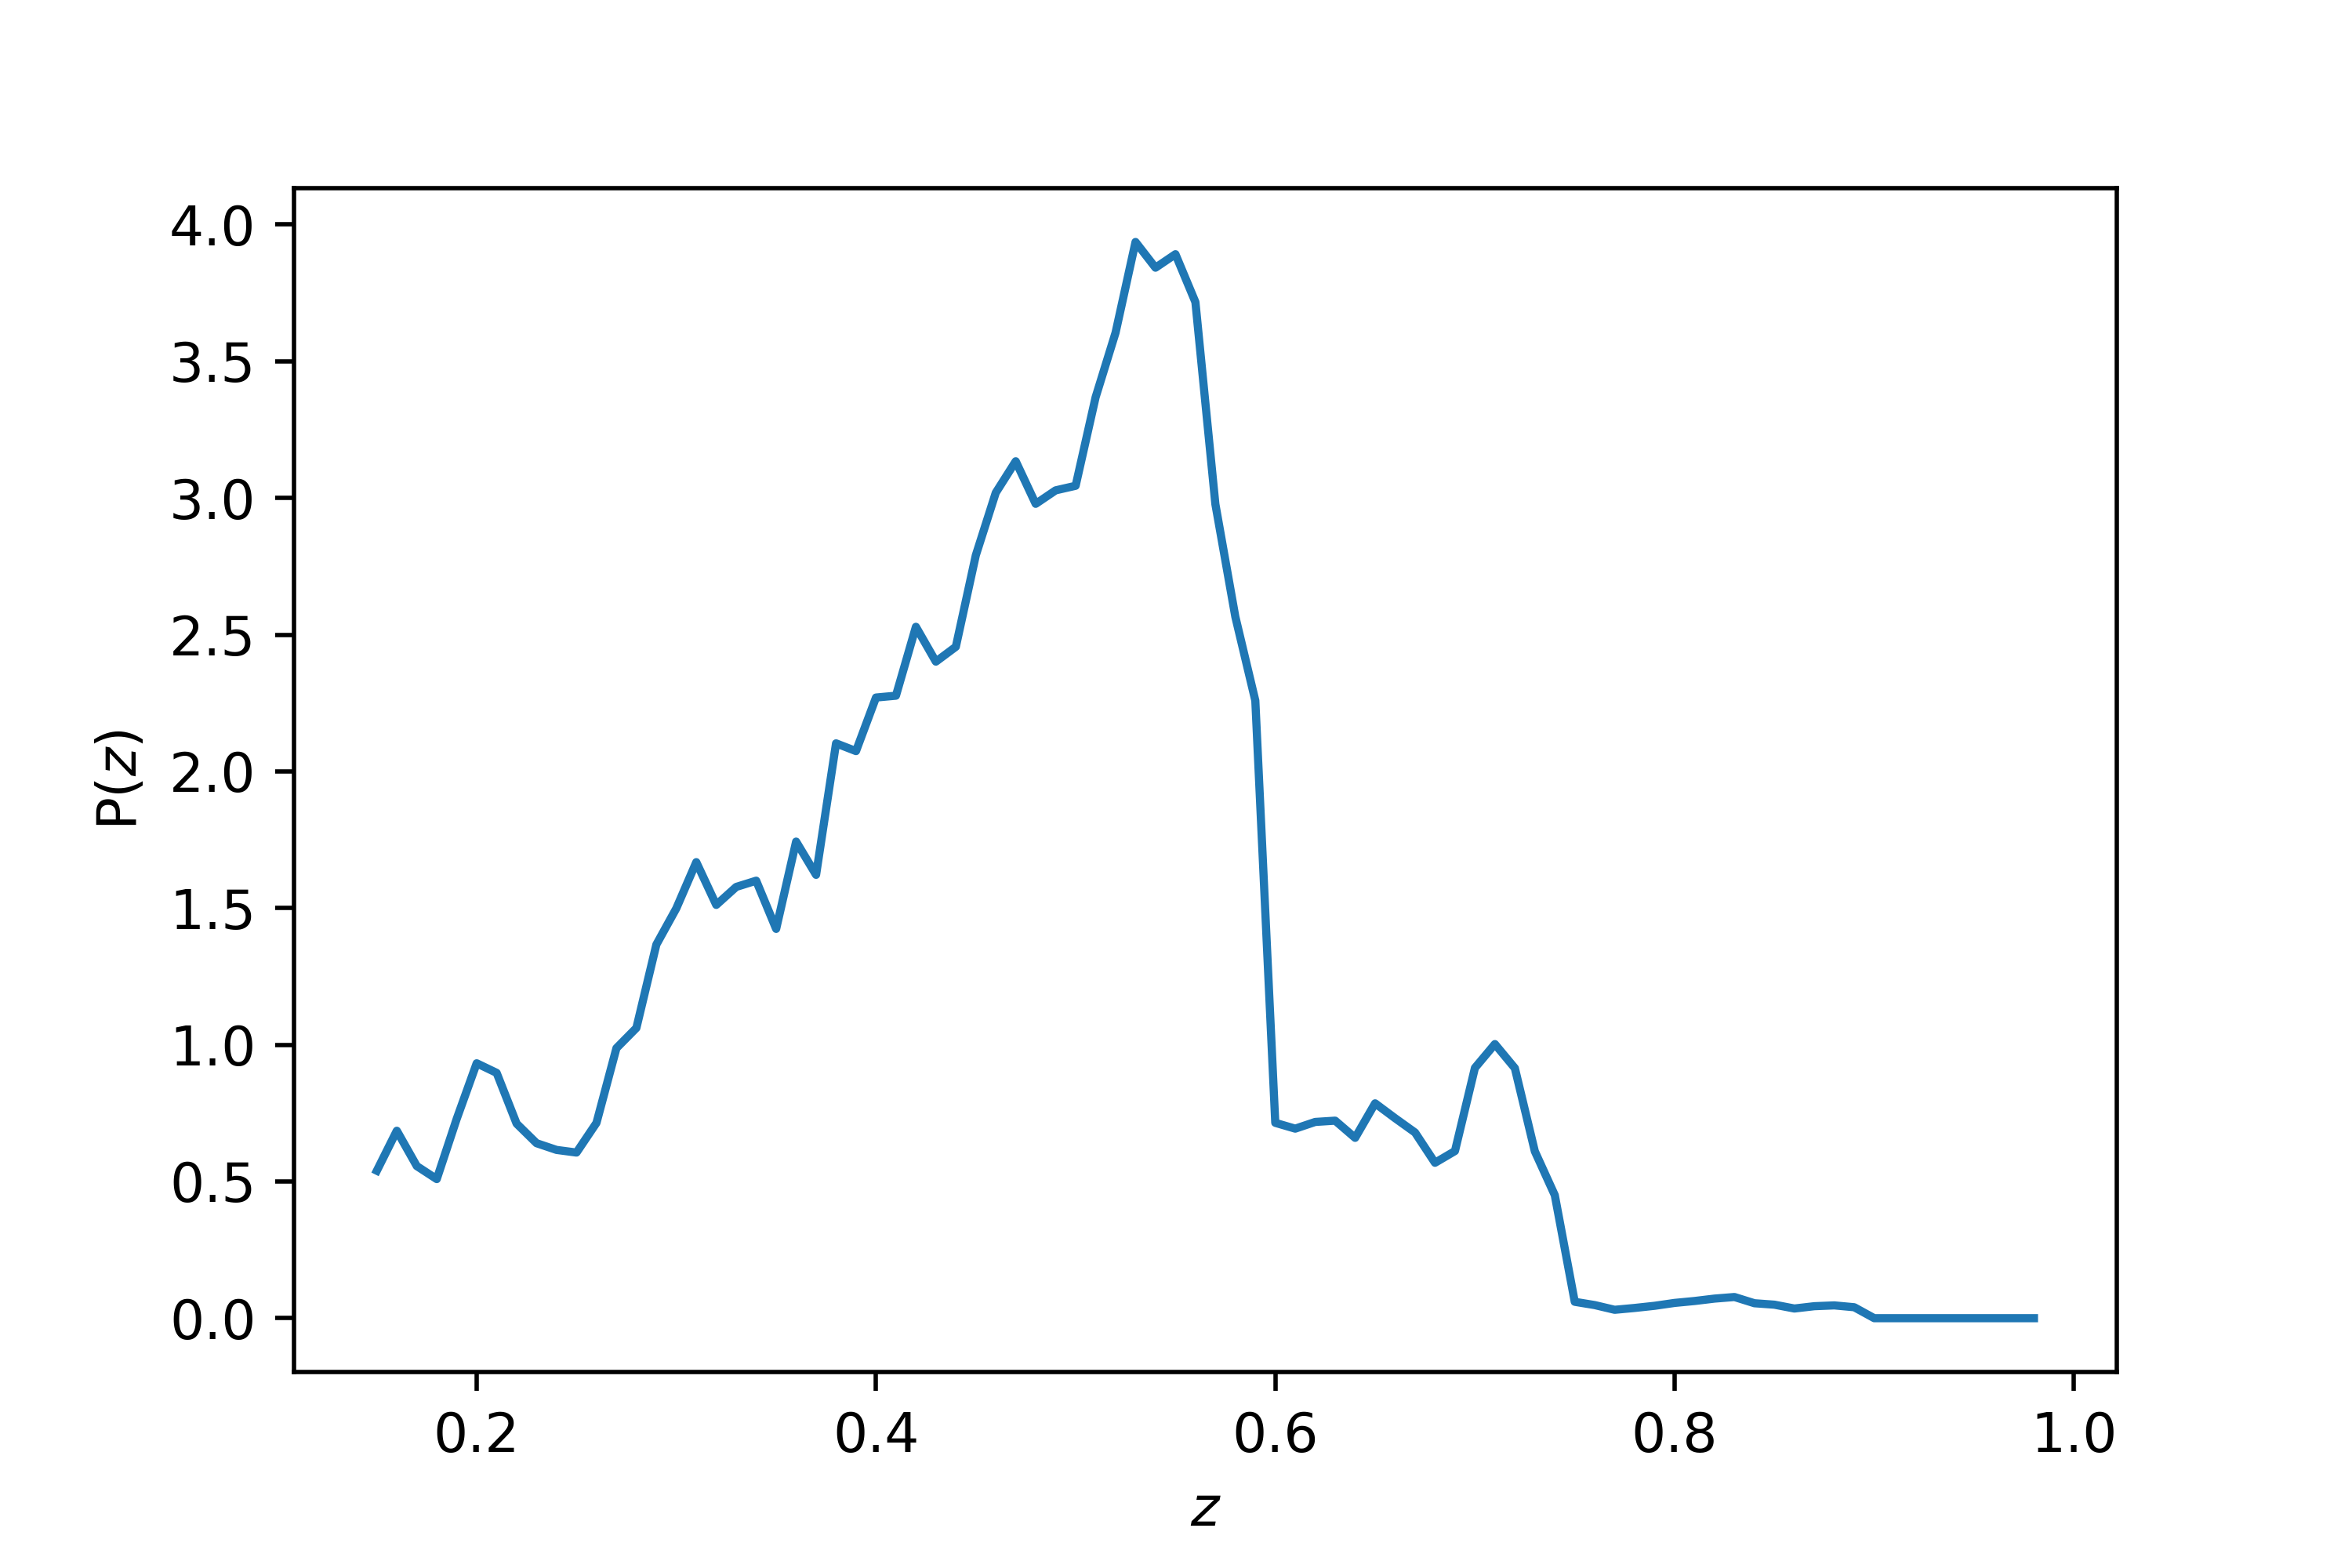
\includegraphics[scale=0.8]{/home/mitchell/Documents/masters/masters/thesis/Ver_2/figures/Redshift_Distribution.png}
\caption{Redshift Distribution of Galaxy Pairs}
\end{figure}



Functionally, this means that the pair is located in the CMB, and a cutout of the CMB is taken around them. They are then rotated, so they are all aligned along the same axis. This subsequent image is then rescaled, so that each pair is located at the same point in the image. They are then added together. 
